%%%%%%%%%%%%%%%%%%%%%%%%%%%%%%%%%%%%%%%%%
% Masters/Doctoral Thesis
% LaTeX Template
% Version 1.43 (17/5/14)
%
% This template has been downloaded from:
% http://www.LaTeXTemplates.com
%
% Original authors:
% Steven Gunn
% http://users.ecs.soton.ac.uk/srg/softwaretools/document/templates/
% and
% Sunil Patel
% http://www.sunilpatel.co.uk/thesis-template/
%
% License:
% CC BY-NC-SA 3.0 (http://creativecommons.org/licenses/by-nc-sa/3.0/)
%
% Note:
% Make sure to edit document variables in the Thesis.cls file
%
%%%%%%%%%%%%%%%%%%%%%%%%%%%%%%%%%%%%%%%%%

%----------------------------------------------------------------------------------------
%	PACKAGES AND OTHER DOCUMENT CONFIGURATIONS
%----------------------------------------------------------------------------------------

\documentclass[11pt, oneside]{Thesis} % The default font size and one-sided printing (no margin offsets)

\usepackage{listings} % Wenn man Code Listings benutzen will mit z.B. \begin{lstlisting}[language=Java] ... \end{lstlisting}
\usepackage{color}
\usepackage{gensymb}
\usepackage[usenames,dvipsnames,svgnames,table]{xcolor}
\definecolor{lightgray}{rgb}{.9,.9,.9}
\definecolor{darkgray}{rgb}{.4,.4,.4}
\definecolor{purple}{rgb}{0.65, 0.12, 0.82}

\renewcommand{\lstlistlistingname}{Quellcodeverzeichnis}
\renewcommand{\lstlistingname}{Quellcode}

\lstdefinelanguage{JavaFXScript}{
  keywords={typeof, new, true, false, catch, function, return, null, catch, switch, var, if, in, while, do, else, case, break},
  keywordstyle=\color{blue}\bfseries,
  ndkeywords={class, export, boolean, throw, implements, import, this},
  ndkeywordstyle=\color{darkgray}\bfseries,
  identifierstyle=\color{black},
  sensitive=false,
  comment=[l]{//},
  morecomment=[s]{/*}{*/},
  commentstyle=\color{purple}\ttfamily,
  stringstyle=\color{red}\ttfamily,
  morestring=[b]',
  morestring=[b]"
}

\lstdefinelanguage{Java}{
  keywords={package, import, public, private, class, extends, implements, void, throws, new, null, int, double, long, String, this, static, interface, abstract},
  keywordstyle=\color{blue}\bfseries,
  identifierstyle=\color{black},
  sensitive=false,
  comment=[l]{//},
  morecomment=[s]{/*}{*/},
  commentstyle=\color{gray}\ttfamily,
  stringstyle=\color{Green}\ttfamily,
  morestring=[b]',
  morestring=[b]"
}

\usepackage{bibgerm} % Wenn man ein Literaturverzeichnis nach der Deutschen Norm haben will
%\usepackage[square, comma]{natbib} % Use the natbib reference package - read up on this to edit the reference style; if you want text (e.g. Smith et al., 2012) for the in-text references (instead of numbers), remove 'numbers'
\hypersetup{urlcolor=blue, colorlinks=true} % Colors hyperlinks in blue - change to black if annoying

\newcommand{\thesisTitle}{Dokumententitel}
\newcommand{\authorName}{Student}

% PDF meta-data
\hypersetup{pdftitle=\thesisTitle}
\hypersetup{pdfauthor=\authorName}

\begin{document}

\frontmatter % Use roman page numbering style (i, ii, iii, iv...) for the pre-content pages

\setstretch{1.5} % Line spacing of 1.5

% Define the page headers using the FancyHdr package and set up for one-sided printing
\fancyhead{} % Clears all page headers and footers
\rhead{\thepage} % Sets the right side header to show the page number
\lhead{} % Clears the left side page header

\pagestyle{fancy} % Finally, use the "fancy" page style to implement the FancyHdr headers

\newcommand{\HRULE}{\rule{\linewidth}{0.5mm}} % New command to make the lines in the title page
\newcommand{\HRule}{\rule{\linewidth}{0.1mm}} % New command to make the lines in the title page

%----------------------------------------------------------------------------------------
%	TITLE PAGE
%----------------------------------------------------------------------------------------

%----------------------------------------------------------------------------------------
%	TITLE PAGE
%----------------------------------------------------------------------------------------

\begin{titlepage}

%top
\begin{center}


\includegraphics[width=0.3\textwidth]{images/TH_Koeln_Logo.png}\\

\vspace*{1cm}

\begin{Huge}
Praxisprojekt\\
\end{Huge}

\vspace*{0.5cm}

\begin{LARGE}
Ermittlung relevanter Themengebiete für die Entwicklung eines Tools zur Unterstützung beim Erstellen von Gestaltungslösungen im Hochschulkontext
\end{LARGE}

\vspace*{1.5cm}

\begin{large}
	von\\
    Christian Alexander Poplawski - 11088931\\

\vspace{1.0cm}

	an der Technology, Arts and Sciences TH Köln\\
    Campus Gummersbach\\
    im Studiengang Medieninformatik (Bachelor)\\

\vspace{1.0cm}

    \begin{tabular}{rl}
        Betreuer:  &  Prof. Dipl. Des. Christian Noss\\
       			   &  \small Technology, Arts and Sciences TH Köln \\[1.0em]

	\end{tabular}

\end{large}

\vspace{1.5cm}

Technology, Arts and Sciences TH Köln, \today \\


\vfill
\end{center}

\end{titlepage}


%----------------------------------------------------------------------------------------
%	ABSTRACT PAGE
%----------------------------------------------------------------------------------------

%----------------------------------------------------------------------------------------
%	ABSTRACT PAGE
%----------------------------------------------------------------------------------------
\thispagestyle{plain}

\addtotoc{Abstract} % Add the "Zusammenfassung" page entry to the Contents

\begin{huge}
	\textbf{Abstract}\\
\end{huge}

Hier steht später das Abstract.

\clearpage

%----------------------------------------------------------------------------------------
%	LIST OF CONTENTS
%----------------------------------------------------------------------------------------

\pagestyle{fancy} % The page style headers have been "empty" all this time, now use the "fancy" headers as defined before to bring them back
\hypersetup{linkcolor=black}
\lhead{\emph{Inhaltsverzeichnis}} % Set the left side page header to "Inhaltsverzeichnis"

\tableofcontents % Write out the Table of Contents

\clearpage

%----------------------------------------------------------------------------------------
%	LIST OF FIGURES/TABLES PAGES
%----------------------------------------------------------------------------------------

%----------------------------------------------------------------------------------------
%	LIST OF FIGURES/TABLES PAGES
%----------------------------------------------------------------------------------------

\pagestyle{fancy} % The page style headers have been "empty" all this time, now use the "fancy" headers as defined before to bring them back

\lhead{\emph{Abbildungsverzeichnis}} % Set the left side page header to "List of Figures"
\addtotoc{Abbildungsverzeichnis} % Add the "Abbildungsverzeichnis" page entry to the Contents
\listoffigures % Write out the List of Figures
\addtocontents{toc}{\vspace{-0.5cm}} % Add a gap in the Contents, for aesthetics

\lhead{\emph{Quellcodeverzeichnis}} % Set the left side page header to "List of Tables"
\addtotoc{Quellcodeverzeichnis}
\lstlistoflistings 
\addtocontents{toc}{\vspace{-0.5cm}}

\clearpage

%\lhead{\emph{Tabellenverzeichnis}} % Set the left side page header to "List of Tables"
%\addtotoc{Tabellenverzeichnis} % Add the "Tabellenverzeichnis" page entry to the Contents

%\addtocontents{toc}{\vspace{0.5cm}} % Add a gap in the Contents, for aesthetics
%\addtocontents{toc}{\vspace{-0.5cm}} % Add a gap in the Contents, for aesthetics
%\listoftables % Write out the List of Tables


%----------------------------------------------------------------------------------------
%	ABBREVIATIONS
%----------------------------------------------------------------------------------------

%----------------------------------------------------------------------------------------
%	ABBREVIATIONS
%----------------------------------------------------------------------------------------

\clearpage % Start a new page

\thispagestyle{plain}

\setstretch{1.5} % Set the line spacing to 1.5, this makes the following tables easier to read

\lhead{} % Set the left side page header to ""

\addtotoc{Abkürzungsverzeichnis} % Add the "Abkürzungsverzeichnis" page entry to the Contents
\begin{huge}
	\textbf{Abkürzungsverzeichnis}\\
\end{huge}

%\lhead{\emph{Abkürzungsverzeichnis}} % Set the left side page header to "Abkürzungsverzeichnis"

\begin{tabular}{ l l }
    \textbf{AWT} & Abstract Window Toolkit\\
    \textbf{API} & Application Programming Interface\\
    \textbf{EDT} & Event Dispatch Thread\\
    \textbf{F3} & Form Follows Function\\
    \textbf{HLS} & HTTP Live Streaming\\ 
    \textbf{RIA} & Rich Internet Application\\    
    \textbf{UI} & User Interface\\    
\end{tabular}


%----------------------------------------------------------------------------------------
%	THESIS CONTENT - CHAPTERS
%----------------------------------------------------------------------------------------

\mainmatter % Begin numeric (1,2,3...) page numbering


\pagestyle{fancy} % Return the page headers back to the "fancy" style

% Include the chapters of the thesis as separate files from the Chapters folder
% Uncomment the lines as you write the chapters

% Chapter 1

%\footnote{vgl. \cite{studie}}

\newcommand{\chaptertitle}{Einleitung}

\chapter{\chaptertitle} % Main chapter title

\label{Einleitung} % For referencing the chapter elsewhere, use \ref{Chapter1} 

\lhead{\chaptername{} \thechapter{} - \emph{\chaptertitle}} % This is for the header on each page - perhaps a shortened title

%----------------------------------------------------------------------------------------

\section{Einleitung}

%----------------------------------------------------------------------------------------

\section{Aktueller Forschungsstand}

%----------------------------------------------------------------------------------------

\section{Themenrelevanz}

%----------------------------------------------------------------------------------------

\section{Aufbau und Methodik}

%----------------------------------------------------------------------------------------

\clearpage
% Chapter 2

\chapter{Ermittlung relevanter Themengebiete} % Main chapter title

\label{Ermittlung} % For referencing the chapter elsewhere, use \ref{Chapter1}

\lhead{\chaptername{} \thechapter{} - \emph{Ermittlung relevanter Themengebiete}} % This is for the header on each page - perhaps a shortened title

%----------------------------------------------------------------------------------------

Für die Ermittlung der relevanten Themengebiete musste zunächst eine geeignete Methode gefunden werden. Hierfür kamen verschiedene Ansätze in Frage.

Ein möglicher Ansatz orientiert sich an einer von einer qualifizierten Person bereits definierten Liste von Inhalten, beispielsweise an einem Buch oder einem Studienverlaufsplan.
Dieser Ansatz gewährleistet durch die Fähigkeiten der Ersteller zum Einen und die große Auswahl von Materialien und damit hohe Vergleichbarkeit zum Anderen einen gewissen Grad von Fehlerfreiheit.
Die definierten Inhalte richten sich jedoch zumeist an Personen, deren Haupttätigkeit die visuelle Gestaltung ist. Bei Verwendung dieser Methode müssen also die Menge und Tiefe der Inhalte kritisch geprüft werden.

Ein weiterer Ansatz orientiert sich am Workflow der Benutzer und beschäftigt sich zunächst mehr mit der Frage nach dem \textit{Wann} als mit der nach dem \textit{Was}. Der Ansatz würde sich also daran orientieren, wann ein Benutzer eine bestimmte Tätigkeit ausführt und welche Art der Unterstützung an dieser Stelle vom Tool einzubringen ist.
Dieser Ansatz wurde schnell als ungeeignet verworfen, da mit ihm ein hoher Aufwand in der Recherche von Arbeitsabläufen der Nutzer einher geht.

Für die Ermittlung wurde schlussendlich ein Fehlerorientierter Ansatz verwendet. Bei diesem Ansatz wurden Artefakte auf die Fehler hin untersucht, die Nutzer häufig machen, und die Inhalte des Tools daraufhin angepasst.
Die Wahl dieser Methode liegt gerade deshalb nahe, weil das Tool zunächst im Hochschulkontext Verwendung finden sollte. Durch das Mediawiki des Studienganges Medieninformatik war der Zugriff auf viele Materialien gewährleistet, die auf Fehler hin untersucht werden konnten. Weiterhin konnte das Tools mithilfe dieses Ansatzes so genau wie möglich auf die Themengebiete spezialisiert werden, in denen die Nutzer häufig Defizite aufzeigen.

%----------------------------------------------------------------------------------------

\section{Vorgehen}
Im ersten Schritt wurden, vorrangig im Mediawiki des Studienganges Medieninformatik, Materialien gesammelt. Um sowohl das Sommer- als auch das Wintersemester und somit alle angebotenen Module abzubilden, wurden alle Dateien untersucht, die im Zeitraum des vergangenen Jahres hochgeladen wurden.
Da nicht jedes der in der Medieninformatik angebotenen Module das Mediawiki verwendet, wurde versucht auch außerhalb des Wikis Materialien zu finden. Hier gestaltete sich die Suche allerdings weitaus aufwendiger und weniger erfolgreich.
Insgesamt wurde ein Katalog von 448 Dateien erstellt, die zur Orientierung zunächst grob in die vier Kategorien \textit{Präsentation, Plakat, Interaktiv} und \textit{Text} unterteilt wurden.

Zur Gruppe \textit{Interaktiv} sei hier angemerkt, dass diese bewusst weit gefasst ist. Sie umfasst sowohl Android-Apps, als auch Websites mit Fokus auf Front- oder Backend.
Eine weitere Unterteilung wurde als nicht Sinnvoll erachtet. So hätten Plattformspezifische Fehler zwar besser gefunden werden können, jedoch soll sich das Tool eher mit gestalterischen Grundlagen befassen und ein möglichst weites Spektrum abdecken. (Weitere Erläuterungen zu den mobilen Plattformen finden sich im Abschnitt \ref{Mobile Plattformen} auf Seite \pageref{Mobile Plattformen})

Die genauen Zahlen der Artefakte in den jeweiligen Kategorien können Tabelle \ref{table:types} auf Seite \pageref{table:types} entnommen werden. Bei der Betrachtung der Werte fällt auf, dass nahezu 50\% der untersuchten Artefakte in die Kategorie “Text” fallen. Weiterhin fällt auf, dass Plakate mit einem Anteil von etwa 3\% aller Artefakte kaum vorhanden waren.

\begin{table}[]
\centering
\begin{tabular}{|l|c|}
\hline
\textbf{Typ} & \multicolumn{1}{l|}{\textbf{Anzahl der Dateien}} \\ \hline
Präsentation & 96                                               \\ \hline
Plakat       & 16                                               \\ \hline
Interaktiv   & 113                                              \\ \hline
Text         & 223                                              \\ \hline
\end{tabular}
\caption{Auflistung der untersuchten Artefakte nach Typ}
\label{table:types}
\end{table}

Das gesammelte Material wurde im nächsten Schritt auf Fehler in der Gestaltung untersucht. Nachfolgend findet sich eine Liste der gefundenen Fehler (in absteigender Reihenfolge nach, Häufigkeit ihres Auftretens):

\begin{itemize}
	\item Fehler beim Einsatz von Farben: Es wurden Farbkombinationen verwendet, die flimmerten, visuell anstrengende Farben wurden als Hintergrundfarbe für Texte gewählt, unharmonische Farbkombinationen, übermäßiger Einsatz von Farben.
	\item Fehlendes raster: Beim Ausrichten der Elemente wurde kein Raster verwendet, Elemente wirken dadurch wie zufällig platziert.
	\item Zu wenig Weissraum: In der Gestaltung wurde zu wenig Whitespace verwendet, die gesamte Gestaltung ist dadurch unübersichtlich und wirkt unruhig.
	\item Visuell anstrengende Tabellen: In Tabellen wurden mehr Trennlinien als nötig verwendet, es wurden zu viele/unpassende Farben verwendet, es war schwer, die Informationen aus der Tabelle zu entnehmen, es wurden Tabellen an unnötigen Stellen verwendet.
	\item Hierarchie im Text nicht deutlich: Die Unterscheide zwischen verschiedenen Elementen (z.B. Überschriften verschiedener Ordnungen) waren zu gering, es wurde keine klare Hierarchie deutlich.
	\item Fehlerhafte Ausrichtung von Elementen: Elemente wurden in sich unsauber ausgerichtet.
	\item Interaktive Elemente nicht deutlich: Es wurde nicht deutlich, mit welchen Elementen der Benutzer interagieren kann und mit welchen nicht.
	\item Bilder gestreckt/gestaucht/verpixelt
	\item Inkonsistente Größen: Gleiche Elemente waren verscheiden groß.
	\item Elementgrößen unverhältnismäßig: Einige Elemente sind im Vergleich zu anderen Elementen unverhältnismäßig zu klein/zu groß.
	\item Zu wenig Kontrast im Text: Text war wegen des Kontrastes schwer lesbar.
	\item Boxes in Boxes: Unnötiges Verwenden von Boxen.
	\item Zeilenhöhe zu groß/klein
	\item Fehler im Textsatz: Vor allem Lücken im Blocksatz
	\item Rechtschreibfehler
	\item Schlecht lesbare Schriftfamilie
\end{itemize}


Abschließend wurde jedem der Fehler eine Oberdisziplin zugeordnet. Auch im Hinblick auf die zur Verfügung stehende Projektzeit wurden darauf aufbauend die Themengebiete definiert, die das Tool abdecken soll:
\begin{itemize}
	\item Typographie
	\item Layout \& Struktur
	\item Whitespace
	\item Farben
	\item Interaktive Elemente
	\item Bilder
\end{itemize}


%----------------------------------------------------------------------------------------

\section{Kritische Reflexion}
Auch wenn dieses fehlerorientierte Vorgehen für das Projekt sehr hilfreich ist, bringt es einige Gefahren mit sich, die hier kurz diskutiert werden sollen.

So ist das Material von nur zwei Semestern keineswegs dazu geeignet, empirische Ergebnisse zu liefern. Die erarbeiteten Ergebnisse liefern lediglich einen Überblick über die Fehler, die in naher Vergangenheit vorherrschend waren. Inhalte von Modulen ändern sich häufig von Semester zu Semester, eine Untersuchung im nächsten Jahr würde also mit hoher Wahrscheinlichkeit andere Fehler zeigen.

Weiterhin wurde nicht für jedes angebotene Modul auch passendes Material gefunden. Es ist also durchaus möglich, dass hier Fehler überhaupt nicht entdeckt wurden.

Als Startpunkt für das Projekt ist die oben aufgeführte Liste jedoch durchaus geeignet.


%----------------------------------------------------------------------------------------

\section{Mobile Plattformen} \label{Mobile Plattformen}
Die mobilen Plattformen, \textit{Android} und \textit{iOS}, die im Studiengang Medieninformatik verwendet werden, besitzen eigene Design Guidelines, die für bestimmte Themengebiete schon Vorgaben und Richtlinien bereit stellen. So legen sowohl die Guidelines für Android als auch für iOS die Verwendung einer oder mehrerer bestimmter Schriftfamilien nahe.

Da sich dieses Tool nicht über die plattformspezifischen Richtlinien hinwegsetzen soll, sollte von Anfang an die Plattform, für die der Nutzer gestaltet, bekannt sein. Die Inhalte des Tools sollten sich dementsprechend anpassen.

%----------------------------------------------------------------------------------------

\clearpage

% Chapter 3

\chapter{Typographie} % Main chapter title

\label{Typographie} % For referencing the chapter elsewhere, use \ref{Chapter1}

\lhead{\chaptername{} \thechapter{} - \emph{Typographie}} % This is for the header on each page - perhaps a shortened title

%----------------------------------------------------------------------------------------

Das Kapitel Typographie könnte als eines der wichtigsten Kapitel dieses Projektes beschrieben werden. Typographie kommt in fast jeder Art von Artefakt vor und bildet den Grundstein einer guten Gestaltung. Gerade weil Typographie jdeoch in so vielen Gebieten Anwendung findet, kann hier unmöglich jeder dieser Anwendungsfälle abgedeckt werden.
Das Projekt befasst sich deshalb auf einem grundlegenden Niveau mit der Typographie und bietet einen Leitfaden zur Erstellung von Fließtexten. Ziel soll es sein, mit Hilfe des Tools einen gut gesetzten und lesbaren Text erstellen zu können.
Anwendungsfälle mit sehr speziellen Ansprüchen an die Typographie, wie zum Beispiel Plakate, werden hier bewusst nicht gesondert angesprochen.

\section{Schriftarten}
Um einen Text zu setzen, müssen eine Reihe von Entscheidungen getroffen werden. Die erste dieser Entscheidungen stellt die Wahl der Schriftart dar.
Schriftarten werden in Kategorien unterteilt, die nicht immer einheitlich sind. So verwendet Strizver \cite{strizver2014type} andere Gruppierungen als  die \textit{British Standards Classification of Typefaces} \cite[S. 51]{baines2005type}. Die zwei Gruppierungen \textit{serif} und \textit{serifenlos} finden sich jedoch in jeder Art der Gruppierung wieder und besonders diese sollen im Rahmen des Projektes betrachtet werden.
Zwar haben auch andere Schriftarten ihre Daseinsberechtigung und Anwendungsfälle, werden jedoch aufgrund der Zielsetzung, einen gut lesbaren Fließtext zu erzeugen, nicht behandelt.

Die Frage, die es zu beantworten gilt, ist also: Sollte das Tool dem Benutzer eine serife oder eine serifenlose Schriftart empfehlen?

Je nach Medium lassen sich in der Lesegeschwindigkeit bei serifen und serifenlosen Schriftarten Unterschiede feststellen, so kommen sowohl \cite{josephson2008keeping} als auch \cite{dogusoy2016serif} zu dem Ergebnis, dass serifenlose Schriftarten an Computerbildschirmen besser gelesen werden können. Serife Schriftarten lassen sich hingegen auf Papier, für das sie ursprünglich entwickelt wurden, besser lesen.
Anzumerken ist hierbei jedoch, dass die Unterschiede in der Lesegeschwindigkeit marginal sind ein gut gesetzter Text in jeder der beiden Schriftarten auch gut lesbar ist.
Weiterhin hängt die Lesegeschwindigkeit davon ab, ob der Leser die Schriftfamilie bereits kennt und ob diese explizit für das verwendete Medium entwickelt wurde. \cite{josephson2008keeping}

Eine allgemeine Empfehlung für die Verwendung von serifen oder serifenlosen Schriftarten lässt sich also nicht abgeben. Vielmehr sollte bei einer Empfehlung darauf geachtet werden, dass die Schriftfamilie für das jeweilige Medium entwickelt wurde und dass eine hohe Chance besteht, dass sie dem späteren Leser des Textes bereits bekannt ist.


%----------------------------------------------------------------------------------------

\section{Schriftfamilien}
Für die Empfehlung einer Schriftfamilie finden sich, wie im vorherigen Kapitel bereits angesprochen, einige Ansatzpunkte. 
So könnte dem Nutzer nahe gelegt werden, eine Schriftfamilie zu verwenden, die speziell für sein Zielmedium entwickelt wurde. Für Computerbildschirme würde sich beispielsweise \textit{Verdana} anbieten, für Printmedien \textit{Times New Roman}.

Ein anderer Ansatz ist die Verwundung von Schriftfamilien, die dem späteren Leser bereits bekannt sind. Die Webseite \textit{www.cssfontstack.com} \cite{cssfontstack} führt eine Liste mit der Verfügbarkeit von Schriftfamilien auf verschiedenen Betriebssystemen, die einen möglichen Orientierungspunkt darstellt. So sind die serifenlosen Schriftfamilien \textit{Arial, Tahoma, TrebuchetMS} und \textit{Verdana} und die serifen Schriftfamilien \textit{Georgia, Palatino} und \textit{Times New Roman} auf etwa 90\% aller Betriebssysteme vorhanden.
Bei Verwendung dieser Schriftfamilien ist die Chance, dass der spätere Leser mit diesen bereits vertraut ist, recht hoch.

Weitere Schriftfamilien ergeben sich aus den Richtlinien der mobilen Plattformen \textit{Android} und \textit{iOS}: So legen die Google Material Design Guidelines die Verwendung der Schriftfamilien \textit{Roboto} und \textit{Noto} nahe, die iOS Human Interface Guidelines sprechen sich für die Verwendung der Systemfont \textit{San Francisco} aus.

Aus den verschiedenen Ansätzen ergibt sich eine Liste von 10 Schriftfamilien, deren Verwendung dem Nutzer, je nach Gestaltungskontext, nahe gelegt werden kann:

\begin{itemize}
	\item Verdana
	\item Times New Roman
	\item Arial
	\item Tahoma
	\item TrebuchetMS
	\item Georgia
	\item Palatino
	\item Roboto
	\item Noto
	\item San Francisco
\end{itemize}

\subsection{Mischen von Schriftfamilien}

Häufig entstehen Fehler, die zu schlecht gesetztem Text führen, beim Mischen von Schriftfamilien. Hier müssen verschiedene Regeln beachtet werden, die zum Teil nur auf subjektiver Ebene entschieden werden können: Die Schriftfamilien müssen miteinander harmonisieren, müssen sich aber gleichzeitig deutlich genug voneinander unterscheiden. Da für das Mischen von Schriftfamilien keine genauen Regeln festgehalten werden können, wird das Tool diesen Bereich nicht behandeln und Texte mit nur einer Schriftfamilie setzen.

%----------------------------------------------------------------------------------------

\section{Schriftgrößen}
Wichtig für die Lesbarkeit eines Textes ist neben der Wahl der Schriftart und -familie vor allem die Größe des Textes. Auch hier gibt es nicht die Eine, richtige Größe. Die Wahl der Größe hängt, wie alle anderen Bereiche, stark von dem Medium ab, in dem die Texte gelesen werden.
Einige Eingrenzungen lassen sich dennoch finden, so empfiehlt \cite{Runk200804} für Bildschirme ab 15” eine Schriftgröße von 14px - 16px, \cite{Lehnert201602} spricht von 14px -24px für Bildschirme und 9 - 12pt für gedruckte Materialien.

Zwar muss die Entscheidung über die Schriftgröße immer noch individuell getroffen werden, jedoch lassen sich mit diesen Werten bestimmte Grenzen finden. So sind 36px für einen Fließtext im Web wahrscheinlich zu groß und 4pt für einen gedruckten Text zu klein.

\subsection{Überschriften}
Semantisch betrachtet leiten Überschriften einen neuen Sinnabschnitt in einem Text ein. Damit eine Überschrift ihren Zweck erfüllt, muss sie einige Eigenschaften besitzen:
Es muss deutlich werden, dass mit der Überschrift ein neuer Abschnitt beginnt, sie muss also aus dem normalen Textfluss heraus fallen. Weiterhin muss deutlich werden, zu welchem Abschnitt die Überschrift gehört.

Um die Überschrift aus dem normalen Textfluss hervor zu heben steht sie klassisch in einer eigenen Zeile. Weiterhin sind sie in der Regel größer als der Fließtext oder (meist bei Überschriften niedrigerer Ordnung) in einem anderen Schriftschnitt gesetzt.

Voraussetzung zum Finden einer passenden Überschriftengröße ist also zunächst, dass sie größer sein muss als der Fließtext. Um die Größe der Überschriften zu errechnen bieten sich verschiedene Methoden an.

\subsubsection{Der goldene Schnitt}
Der \textit{goldene Schnitt} findet in vielen Bereichen der visuellen Gestaltung und auch der Natur Anwendung. Er beschreibt ein Verhältnis, das von Menschen in der Regel als harmonisch wahrgenommen wird.
Laut \cite{livio2003golden} wird dieses Verhältnis durch eine unendliche, sich niemals wiederholende Zahl beschreiben. Diese wird im Folgenden mit 1.62 angenähert.

Als erster Ansatz bietet es sich an, die Größe einer Überschrift zu errechnen, indem die Schriftgröße des Fließtextes mit dem goldenen Schnitt multipliziert wird.
Für einen Fließtext mit einer Schriftgröße von 14px würde sich eine Überschriftengröße von \(14px * 1.62 = 22.68px\) ergeben.
Als erster Ansatz scheint diese Methode valide, jedoch bleiben einige Probleme bestehen.

Zum Einen ist 22.68px eine Gleitkommazahl und somit als Schriftgröße nicht sehr schön. Die Zahl ließe sich aufrunden, aber auch 23px sind als Schriftgröße eher unüblich.
Zum Anderen ist mit dieser Methode zwar die Größe für eine Überschrift gefunden, häufig bestehen Texte jedoch aus mehreren Überschriften verschiedener Ordnung.

\subsubsection{Typographic Scale}
Die \textit{Typographic Scale} rührt aus den frühen Zeiten des Buchdruckes, als Texte noch aus einzelnen Buchstaben zusammen gesetzt wurden. Die Auswahl an Schriftgrößen war zu dieser Zeit aus rein technischen Gründen sehr limitiert, die Skala wird aber auch heute noch in vielen Programmen verwendet. Eine Variation diese Typographic Scale kann Abb.X entnommen werden.

\textbf{HIER BILD VON SCALE AUS BUCH}

Die Typographic Scale könnte im ersten Schritt genutzt werden, um die mit dem goldenen Schnitt errechnete Zahl an einen Wert aus der Skala anzunähern.
Die im obigen Beispiel errechnete Größe lautet 22.68px, auf der Typographic Scale liegt sie zwischen den Werten 21 und 24. Da sie näher an der 24 liegt wird 24px als Schriftgröße für die Überschrift gewählt. Das Ergebnis ist zunächst befriedigend und kann Abb. \ref{fig:basicHeadline} auf Seite \pageref{fig:basicHeadline} entnommen werden.

\begin{figure}[h]
    \centering
    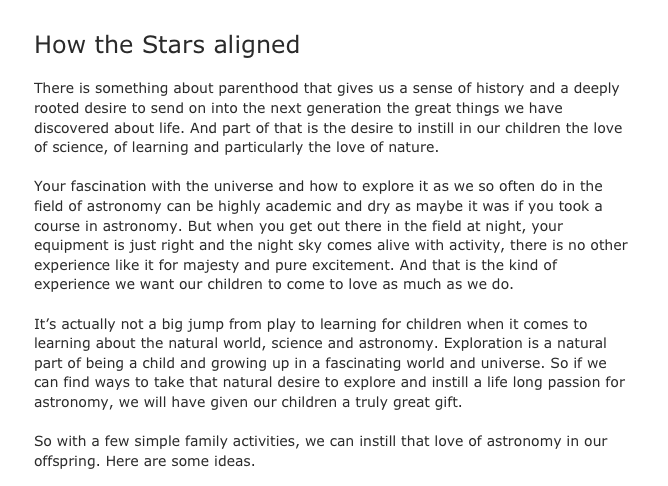
\includegraphics[width=1\textwidth]{images/Proof-Golden-Ratio.png}
    \caption{Text mit 14px Body Schriftgröße und 24px Headline Schriftgröße}
    \label{fig:basicHeadline}
\end{figure}

Das Problem der Überschriften verschiedener Ordnungen ist damit jedoch immer noch nicht gelöst. Jedoch kann zumindest eine begrenzte Menge von Zwischenüberschriften aus den Zwischenschritten von Fleißtext und der oben errechneten Überschrift gebildet werden. Im Fall des obigen Beispiels wären diese Überschriften 21px, 18px und 16px groß (s. Abb. \ref{fig:threeHeadlines} auf Seite \pageref{fig:threeHeadlines}).

\begin{figure}[h]
    \centering
    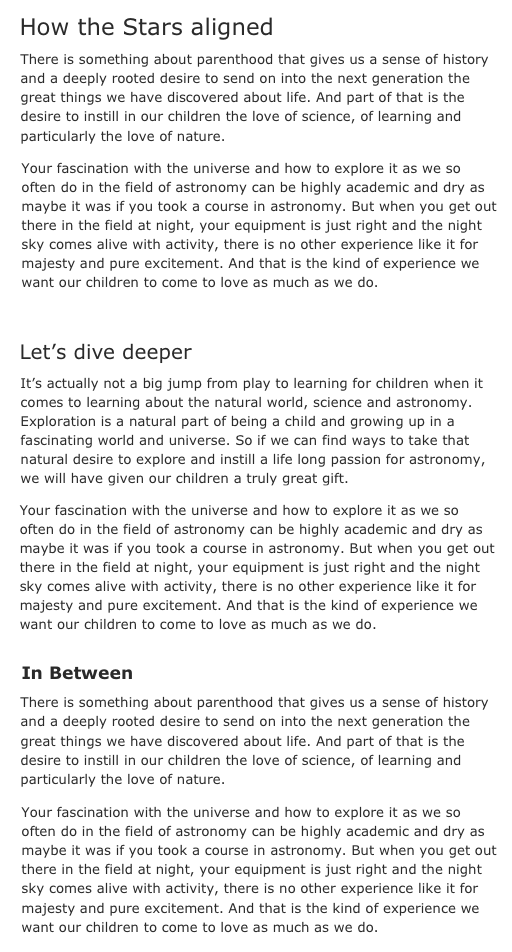
\includegraphics[width=0.7\textwidth]{images/three-headlines.png}
    \caption{Text mit drei Überschriften verschiedener Ordnung}
    \label{fig:threeHeadlines}
\end{figure}


\textbf{HIER ZWEITES BILD VON GESETZTEM TEXT}

Befinden sich eine Überschrift und der Text nur 2px auseinander, so scheint es ratsam, die Überschrift auch anderweitig abzuheben, etwa durch einen fetten Schriftschnitt.

Ein letztes Problem wird bei der Verwendung der Gleichung für nahe aneinander liegende Schriftgrößen deutlich. So wäre die Überschrift erster Ordnung für Fließtexte der Größe 14px, 16px und 18px jeweils 21px.


\begin{equation}
\begin{split}
14px * 1.62 = 22,68px => 24px \\
16px * 1,62 = 25,92px => 24px \\
18px * 1,62 = 29,16px => 24px \\
21px * 1,62 = 34,02px => 36px \\	
\end{split}
\end{equation}


Um die Überschriften weiter zu differenzieren bietet es sich an, eine Konstante mit in die Rechnung einzubeziehen, die zum Wert des goldenen Schnitts addiert wird. Diese errechnet sich aus der Abweichung der Größe des Fließtextes von 14px geteilt durch 10. Bei Schriftgrößen unter 14px wird diese aufgrund der kleineren Abständen zwischen den einzelnen Größen auf der Skala nicht benötigt.
Dieser Wert hat keinen weiteren wissenschaftlichen Hintergrund, vielmehr liefert er für Schriftgrößen zwischen 14px und 24px gut gestaffelte Werte und wird daher verwendet.

Eine angepasste Berechnung unter Berücksichtigung der Konstante liefert befriedigendere Ergebnisse:

\begin{equation}
\begin{split}
14px * 1.62 = 22,68px => 24px \\
16px * (1,62 + 0,2) = 29,12px => 24px \\
18px * (1,62 + 0,4) = 36,36px => 36px \\
21px * (1,62 + 0,7) = 48,72px => 48px \\
\end{split}
\end{equation}


Somit wurde ein verwendbarer Ansatz zur Größenberechnung von Überschriften basierend auf der Größe des Fließtextes gefunden. Dieser Ansatz liefert nur Richtwerte und kann keinesfalls als allgemeingültige Regel verstanden werden. Weiterhin funktioniert er nur für einen bestimmten Bereich an Schriftgrößen. Für die Verwendung  im Rahmen dieses Tools ist er jedoch ausreichend.


%----------------------------------------------------------------------------------------

\section{Abstände im Text}
TBD

\subsection{Zeilenhöhe und -länge}
Für Zeilenhöhe und -länge lassen sich recht genaue Richtwerte finden. Im Print-Bereich wird ein Zeilenabstand von 120\% \cite[S. 150]{Runk200804} als optimal angesehen, das W3C empfiehlt, mit Blick auf Menschen mit Sehbehinderungen, einen Zeilenabstand von 150\% bis 200\% \cite{W3C}. Für die Zeilenlänge legen Studien 65 - 75 CPL (Characters per Line) nahe \cite{bernard2002effects}, die einen guten Lesefluss ermöglichen, ohne die Suche nach dem Anfang der nächsten Zeile zu kompliziert zu machen.
Die Toleranz für die Zeilenhöhe im Tool sollte also bei einem Wert zwischen 120\% und 180\% liegen. Wie hoch genau eine optimale Zeilenhöhe ist, hängt dabei auch von der Schriftart und dem Einsatzgebiet ab, auch bei diesen Werten handelt es sich also nur um eine Empfehlung.

\subsection{Absätze und Überschriften}
Ein Absatz beschreibt einen neuen Sinnabschnitt im Text, der auch visuell erkennbar sein sollte. In der Regel werden zwei Absätze dabei durch eine Leerzeile voneinander getrennt. In Textverarbeitungsprogrammen wie zum Beispiel \textit{Microsoft Word} reicht diese Richtlinie und der Nutzer muss keine eigenen Berechnungen durchführen, beim Verwenden von Grafikprogrammen oder beim erstellen von Websites kann aber eine manuelle Einstellung nötig sein. Die Höhe einer Leerzeile lässt sich durch die Zeilenhöhe berechnen: Bei einer Textgröße von 14px beträgt die Zeilenhöhe \(14 * 140\% = 19,6\) also etwa 20px. Die Höhe einer Leerzeile ist dementsprechend \(20px + 14px = 34px\).

Auch die Abstände der Überschriften lassen sich auf Grundlage der Zeilenhöhe berechnen. Als Grundsatz gilt dabei, dass eine Überschrift näher an dem Absatz platziert sein sollte, den sie betitelt und dass Überschriften höherer Ordnung im vergleich zu denen niedrigerer Ordnung mehr Abstand zum Text besitzen sollten.

Aufbauend auf der obigen Rechnung können für die Abstände der Überschriften Vielfache der Zeilenhöhe verwendet werden, also beispielsweise 40px, 60px und 80px. Diese Werte können nun als Ober- und Unterabstände der jeweiligen Überschriften verwendet werden.

\begin{itemize}
	\item H1: 24px, Top 50px, Bottom 30px (Zeilenhöhe * 4)
	\item H2: 21px, Top 40px, Bottom 20px (Zeilenhöhe * 3)
	\item H3: 18px Bold, Top 30px, Bottom 10px (Zeilenhöhe * 2)
\end{itemize}

Das nachfolgende Bild zeigt einen mit den errechneten Abständen gesetzten Text:

\textbf{HIER NOCH BILD}

An dieser Stelle ist erwähnenswert, dass der Großteil aller Programme diese Abstände auch automatisch setzen, wenn die entsprechenden Elemente auch korrekt ausgezeichnet werden. In der Fehleranalyse wurde jedoch deutlich, dass diese korrekte Auszeichnung häufig versäumt wird.

%----------------------------------------------------------------------------------------

\section{Kontrast}
Zuletzt sollte im Tool auch der Kontrast eines Textes zu dessen Hintergrund behandelt werden, der einen großen Einfluss auf die Lesbarkeit hat.
Nach Möglichkeit sollte es vermieden werden, lange Textpassagen auf einem Farbigen Hintergrund zu platzieren.
Der sicherste (und der wohl auch am häufigsten gewählte) Weg ist, schwarzen Text auf einem weißen Hintergrund zu verwenden. Auch die umgekehrte Zusammensetzung (also Schwarzer Hintergrund und Weißer Text) ist recht unproblematisch.

Bei allen weiteren Kombination muss der Kontrast überprüft werden. Die Überprüfung gestaltet sich dabei jedoch recht simpel, da sowohl für die Berechnung als auch für die Einordnung eines Kontrastes Spezifikationen in den Web Content Accessibility Guidelines des w3c \cite{w3c2016g18} vorhanden sind. Das Tool wird sich an diese halten.

Abschnitt 1.4.3 der Web Content Accessibility Guidelines definiert drei verschiedne Level von Kontrasten, die jeweils die relative Leuchtkraft zweier Farben in ein Verhältnis setzen (\textit{A (3:1), AA(4.5:1), AAA(7:1)}).

In Quellcode \ref{lst:contrast-code} auf Seite \pageref{lst:contrast-code} findet sich eine Umsetzung dieser Rechnung in JavaScript, die aus dem \textit{Proof of Concept} entonmmen ist, der für dieses Kapitel angefertigt wurde.

\begin{lstlisting}[caption={Berechnung des Kontrastverhältnisses zweier Farben nach WCAG 2.0 in JavaScript}, label={lst:contrast-code}, language=javascript]
  // Check contrast of the two currently picked colors
  // based on WCAG 2.0 G18
  // https://www.w3.org/TR/2016/NOTE-WCAG20-TECHS-20160317/G18
  calculateRatio() {
    // Get currently set colors
    let bgColor = hexRgb(this.props.bgColor)
    let fgColor = hexRgb(this.props.fgColor)
    var colors = [bgColor, fgColor];
    var lumis = [];
    var ratio;

    for(var i = 0; i <colors.length; i++) {
      var currColor = colors[i];

      // Convert RGB values of colors to sRGB
      // Then do claculations as specified in WCAG 2.0 G18
      // https://www.w3.org/TR/2016/NOTE-WCAG20-TECHS-20160317/G18#G18-tests
      for (var singleColor in currColor) {
        if (currColor.hasOwnProperty(singleColor)) {
          currColor[singleColor] = currColor[singleColor] / 255;

          if (currColor[singleColor] <= 0.03928) {
            currColor[singleColor] = currColor[singleColor] / 12.92;
          } else {
            currColor[singleColor] = Math.pow(((currColor[singleColor] + 0.055) / 1.055), 2.4);
          }
        }
      }

      // Store luminances of foreground and background color
      lumis.push((0.2126 * currColor[0] + 0.7152 * currColor[1] + 0.0722 * currColor[2]) + 0.05);
    }

    // Normalize luminances so that the darker one is 1
    if(lumis[0] > lumis[1]) {
      var multiplicator = 1 / lumis[1];
      lumis[0] = lumis[0] * multiplicator;
      ratio = lumis[0];
    } else {
      var multiplicator = 1 / lumis[0];
      lumis[1] = lumis[1] * multiplicator;
      ratio = lumis[1];
    }

    return ratio
  };
\end{lstlisting}

%----------------------------------------------------------------------------------------

\clearpage

% Chapter 4

\chapter{Layout und Struktur} % Main chapter title

\label{LayoutStruktur} % For referencing the chapter elsewhere, use \ref{Chapter1}

\lhead{\chaptername{} \thechapter{} - \emph{Layout und Struktur}} % This is for the header on each page - perhaps a shortened title

%----------------------------------------------------------------------------------------

Während der Fehleranalyse konnten immer wieder grundlegende Fehler in der Anordnung von Elementen beobachtet werden, die dazu führten, dass ein Artefakt unsauber wirkte.
Diese Fehler lassen sich mit sehr simplen Mitteln, wie Hilfslinien oder Grid Systems, vermeiden.
Hier unterscheiden sich die verschiedenen Medien und Plattformen im Hinblick auf bestehende Lösungen und mögliche Ansätze, weshalb dieses Kapitel in jeweils spezifische Unterkapitel unterteilt ist.

\section{Grid Systems im Web}
Für Gestaltungen im Web sind Grid Systems sehr verbreitet, nicht zuletzt auch wegen ihres hohen Mehrwertes im Bezug auf Responsive Webdesign.
Wegen der hohen Anzahl bereits bestehender Lösungen liegt es nahe, dass das Tool dem Nutzer nicht beim Erstellen eines eigenen Grid Systems hilft, sondern nur die Grundlagen vermittelt und für die Umsetzung auf eine bereits bestehende Lösung verweist.
Hierfür wurden zunächst verschiedene Grid Systems auf ihre Konfigurationsmöglichkeiten und ihren Output hin untersucht und evaluiert.

\textbf{gridpak} (http://gridpak.com) \\
Geeignet, um individuelle Grid Systems zu erstellen. Sehr simpel, da nur drei Werte verändert werden müssen (plus Option zum Anlegen von Breakpoints). \\
\textit{Output:} Verschiedene CSS und JS Files und das Grid System als png.

\textbf{960px Grid} (http://960.gs) \\
Festes, 960px breites Grid System, keine individuellen Einstellungen mehr Möglich. \\
\textit{Output:} Verschiedene CSS Dateien sowie vorlagen für viele Grafikprogramme.

\textbf{1200px Grid} (https://1200px.com) \\
Aufbauend auf dem 960px Grid, aber 1200px breit. Außerdem in allen Werten anpassbar. \\
\textit{Output:} CSS Dateien oder Photoshop/Illustrator Files.

\textbf{Bootstrap} (http://getbootstrap.com/2.3.2/index.html) \\
Sehr flexibel und anpassbar, allerdings nur, wenn es im Web verwendet wird, Einbindung über HTML/CSS also Pflicht. \\
\textit{Output:} Im Code verwendbare CSS-Klassen.

\textbf{Dead Simple Grid} (https://github.com/mourner/dead-simple-grid) \\
Ähnlich wie Bootstrap aber sehr viel simpler. Flexibel anpassbar, aber ebenfalls nur für die Verwendung mit HTML/CSS geeignet. \\
\textit{Output:} Im Code verwendbare CSS-Klassen.

\textbf{Bourbon Neat} (http://neat.bourbon.io) \\
Ähnlich wie Bootstrap \& Dead Simple Grid aber deutlich komplexer, da es zwingen über einen CSS-Präprozessor eingebunden werden muss. Flexibel anpassbar, aber ebenfalls nur für die Verwendung mit HTML/CSS geeignet. \\
\textit{Output:} Im Code verwendbare CSS-Klassen.

\textbf{Foundation} (http://foundation.zurb.com) \\
Ähnlich wie Bootstrap. Flexibel anpassbar, aber auch nur für HTML/CSS geeignet. \\
\textit{Output:} Im Code verwendbare CSS-Klassen.

\subsection{Abbildung im Tool}
Da sich die untersuchten Grid Systems in ihren Eigenschaften sehr unterscheiden, sollte das Tool mehrere Empfehlen und ihre typischen Einsatzgebiete nennen.
Die Wahl fiel mit gridpack auf ein System, das auch unabhängig vom Code eingesetzt werden kann, sowie auf Foundation, das nur im CSS verwendet werden kann. Foundation wurde gewählt, da es die Möglichkeit bietet, nur das Grid System ohne Klassen für andere Elemente, wie zum Beispiel Buttons, einzubinden.
Um dem Nutzer das Arbeiten mit Grid Systems näher zu bringen, könnte das Tool diesen dazu auffordern, verschiedene Elemente auf einer Seite zu Platzieren. Zunächst sollte die Platzierung ohne eine Hilfestellung stattfinden (s. Abb.X), im zweiten Schritt dann mit einem simplen, vom User konfigurierten Grid System (s. Abb.X).

\section{Grid Systems auf nativen Plattformen}
Auf nativen Plattformen werden Grid Systems eher von Interface Designern verwendet, vorgefertigte Grid Systems  wie sie im Web für die Umsetzung verwendet werden können, bestehen in dieser Art nicht. Die Zielgruppe des Tools besteht jedoch nicht aus Interface Designern, sondern aus Studenten, die Projekte in der Regel in der Rolle des Entwicklers durchführen. Hier müssen also plattformspezifische Grundlagen gefunden werden.

Unter iOS spielt das Storyboard in Xcode für die Platzierung von Elementen eine wichtige Rolle. Im Storyboard ist ein implizites Grid System vorhanden, dass zumindest die Außenabstände und die Abstände von Elementen untereinander mit Hilfslinien kennzeichnet. (s. Abb. \ref{fig:xcode-guides} auf Seite \pageref{fig:xcode-guides})
Das Tool sollte an dieser Stelle auf die Verwendung des Storyboards hinweisen, eine weitere Interaktivität macht wenig Sinn.

\begin{figure}[h]
    \centering
    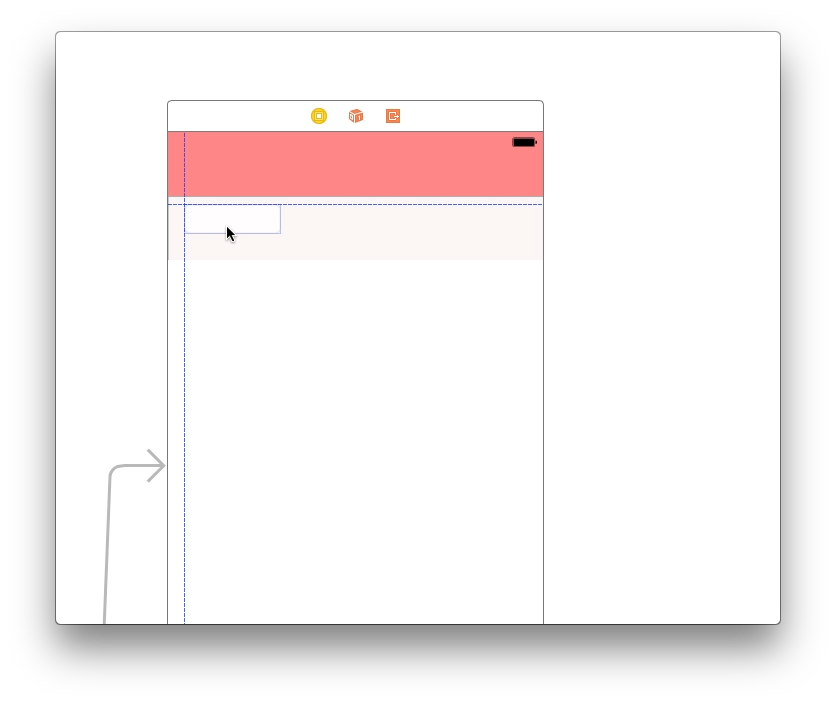
\includegraphics[width=1\textwidth]{images/xcode-guidelines.png}
    \caption{Automatische Guidelines im Xcode Stroyboard}
    \label{fig:xcode-guides}
\end{figure}

Für Android gestaltet sich das erstellen von Layouts schwieriger, da der in Android Studio enthaltene Visuelle Editor deutlich weniger intuitiv ist und weniger Hilfestellung liefert, als die Storyboards von Xcode. Das Interface wird hier in der Praxis außerdem deutlich häufiger in XML-Form beschreiben und nicht durch den visuellen Editor erzeugt. In den Material Design Guidelines wird generell ein 8dp Square Grid verwendet. Das heißt, der Abstand von allen Elementen nach außen beträgt mindestens 8dp, jedoch sind für alle UI-Elemente auch zusätzlich spezifische Abstände angegeben, auf die verwiesen werden sollte. Für alle Elemente und Endgeräte sind außerdem Illustrator-Vorlagen vorhanden. 

\section{Grid Systems in einfachen Texten}
Generell sind Grid Systeme auch im Textsatz-Bereich sehr verbreitet und finden dort sogar ihren Ursprung. Sie unterscheiden sich aber durchaus von Grid-Systemen, wie man sie im Web-Bereich verwendet. Auch hier gibt es verschiedene Ausführungen, so werden horizontale Raster verwendet, um die Ausrichtung der Zeilen über die Seite hinweg zu ordnen oder der Satzspiegel, der die harmonische Platzierung von Text auf einer Doppelseite vereinfacht. \\
Das Tool soll sich aber auf Systeme konzentrieren, die nur wenige Spalten als Platz für den Fließtext verwenden.

Da viele der im Rahmen der Fehleranalyse untersuchten Artefakte einzelne Textseiten (beispielsweise Exposés) waren, wird der Fokus des Tools darauf liegen, eine einzelne Textseite zu setzen.
Hier sind sowohl die Abstände vom Text zum Rand der Seite als auch die Abstände von Spalten untereinander interessant.

Weiterhin sollte erwähnt werden, dass die meisten Textverarbeitungsprogramme diese Abstände bereits in den Standardeinstellungen auf solide Werte setzen und das Tool auch hier eher ein Grundverständnis vermitteln, als eine konkrete Lösung anbieten sollte.

\subsection{Berechnung}
Die simpelste mögliche Berechnung verwendet einen Bruchteil der Gesamtlänge der kürzesten Kante des Dokumentes als Außenabstand. Für ein DIN A4 Blatt mit einer Breite von 595px oder 210mm ergibt sich bei der Verwendung von 10\% der Breite ein Außenabstand von etwa 60px oder 21mm.
Eine so gesetzte Textseite kann Abb. \ref{fig:a4-single-col} auf Seite \pageref{fig:a4-single-col} entnommen werden.

\begin{figure}[h]
    \centering
    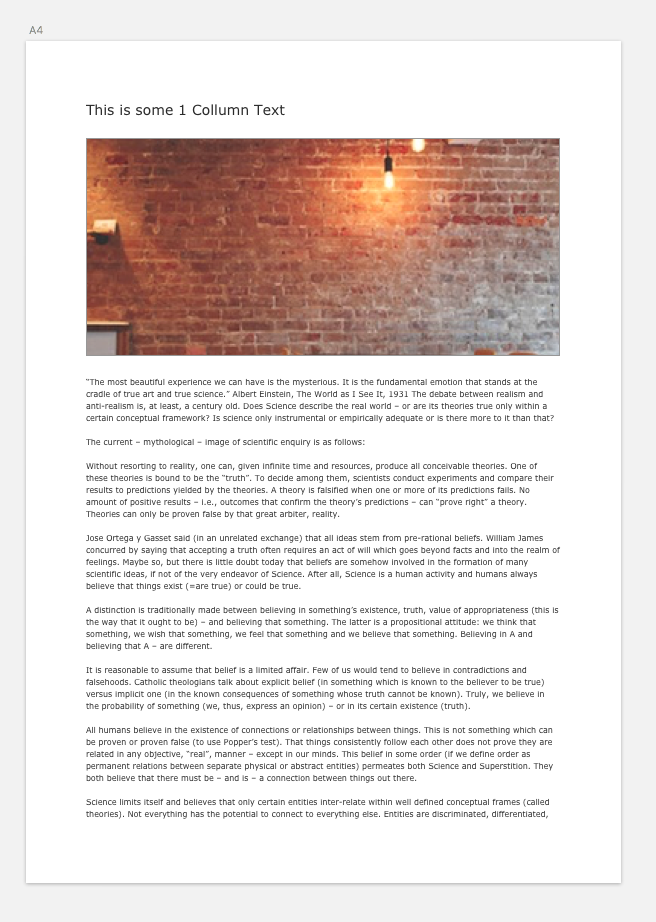
\includegraphics[width=0.5\textwidth]{images/A4-single-col.png}
    \caption{Mit 10\% außenabstand gesetzte DIN-A4 Seite}
    \label{fig:a4-single-col}
\end{figure}

Mit diesem Wert ist zunächst also eine grobe Richtlinie gefunden. Nach unten lassen sich für den Abstand genaue Grenzen finden: Viele Drucker benötigen einen Druckrand von etwa 15mm, das Tool sollten den Nutzer also warnen, sollte der Abstand nach außen diesen Wert unterschreiten.

Sollte ein Layout mit mehr als einer Spalte gewünscht sein, kann der Abstand zwischen diesen Spalten ebenfalls über den errechneten Außenabstand definiert werden. Der Abstand zwischen den Spalten sollte dabei kleiner sein, als der nach außen, es bietet sich also die Hälfte des Außenabstandes an. Mit den oben errechneten Werten wäre der Abstand zwischen zwei Spalten also 30px oder etwa 10mm. Ein mit diesen Werten gesetzter Text kann Abb. \ref{fig:a4-two-col} auf Seite \pageref{fig:a4-two-col} entnommen werden.

\begin{figure}[h]
    \centering
    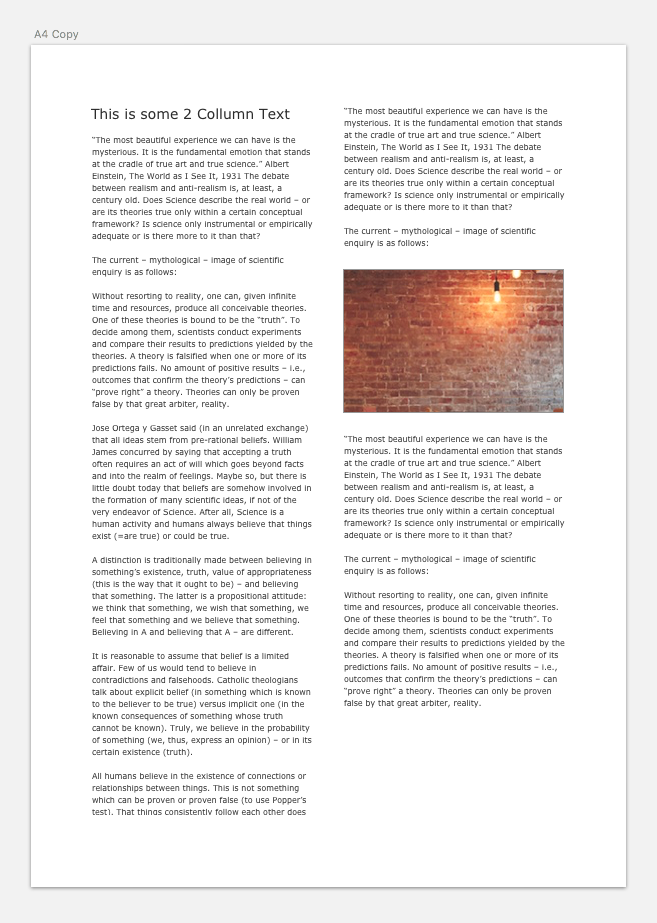
\includegraphics[width=0.5\textwidth]{images/A4-two-col.png}
    \caption{Eine mit zwei Spalten Text und 30px Abstand gesetzte DIN-A4 Seite}
    \label{fig:a4-two-col}
\end{figure}

Zu beachten ist hier, dass die Spalten mit diesen Werten nur jeweils 445px breit wären und hierdurch die im Kapitel Typographie behandelte optimale Laufweite des Textes von 75 - 90 CPL je nach verwendeter Schriftgröße nicht mehr gewährleistet ist. Das Tool sollten die im ersten Schritt errechneten Werte für Texte kennen und den Nutzer auf diesen Umstand hinweisen.

\subsection{Abbildung im Tool}
Das Tool soll dem Nutzer die Möglichkeit geben, ein Format zu wählen. Für dieses Format sollte der User dann die Anzahl der Spalten, die Abstände zwischen den Spalten und die Abstände nach außen einstellen können.
Das Tool weist den Nutzer dann darauf hin, welche Werte aus welchen Gründen kritisch sind.
Optional soll noch ein Bild eingefügt werden können. Die Platzierung soll dem Nutzer überlassen werden und ihn dazu bringen, bereits im Tool auch aktiv mit einem Layout zu arbeiten.

% Chapter 5

\chapter{Whitespace} % Main chapter title

\label{Whitespace} % For referencing the chapter elsewhere, use \ref{Chapter1}

\lhead{\chaptername{} \thechapter{} - \emph{Whitespace}} % This is for the header on each page - perhaps a shortened title

%----------------------------------------------------------------------------------------

Bei den Recherchen im Bereich Whitespace wurde schnell deutlich, dass dieses Gebiet, anders als beispielsweise die Typographie, deutlich weniger konkrete Regeln bietet. Viele der Entscheidungen können nur sehr individuell, von Gestaltung zu Gestaltung, getroffen werden. \\
Die Hauptfrage in diesem Abschnitt ist also zunächst: Gibt es überhaupt konkrete Regeln, auf dessen Basis das Tool arbeiten könnte?

%----------------------------------------------------------------------------------------

\section{Was ist Whitespace?}

Whitespace (auch \textit{negative space} oder \textit{Weissraum}) ist leerer Raum innerhalb einer Gestaltung. Für die Qualität einer Gestaltung spielt dieser eine zentrale Rolle:

\begin{quote}
The single most overlooked element in visual design is emptiness. The lack of attention it receives explains the abundance of ugly and unread design. [...]
Design elements are always viewed in relation to their surroundings. Emptiness in two-dimensional design is called white space and lies behind the type and imagery. But it is more than just the background of a design, for if a design's background alone were properly constructed, the overall design would immediately double in clarity and usefulness. Thus, when it is used intriguingly, white space becomes foreground. The emptiness becomes a positive shape and the positive and negative areas become intricately linked. \cite[S.19]{white2011elements}
\end{quote}

Whitespace ist also kein Raum, den es noch zu füllen gilt, sondern bewusst leer gelassener Raum, dessen Aufgabe es ist, Elemente in ihrer Wichtigkeit zu unterstützen. \\
Eine erste, recht ungenaue Regel die sich aufstellen lässt ist die, dass wichtige Elemente mehr Weissraum um sich haben als weniger wichtige. Diese Regel wurde beispielsweise in der Typographie angewendet: Überschriften höherer Ordnung haben im Gegensatz zu denen niedrigerer Ordnung größere Abstände zum Text.

Weiterhin lässt sich feststellen, dass eine Gruppe von Elementen, die dem Gesetz der Nähe \cite{mayer2005einfuhrung} unterliegt, zueinander weniger Whitespace aufweist, als nach außen.

Genaue Werte, wie groß Abstände im Verhältnis zu Elementen sein müssen, um ästhetisch ansprechend zu wirken, lassen sich jedoch nicht finden. Auch Konsistenzen im Weißraum sind schwer zu definieren. So haben Elemente häufig andere horizontale als vertikale Abstände, oft sind selbst die Abstände nach oben und unten verschieden. \\
Das Tool kann an dieser Stelle also nur grobe Regeln im Umgang mit Whitespace vermitteln. Eine Interaktivität ließe sich zum Beispiel in der Gruppierung von Elementen oder dem Bilden einer Hierarchie mittels Whitespace schaffen. Weiterreichende Möglichkeiten zur interaktiven Vermittlung von Inhalten konnten nicht gefunden werden. Das Kapitel Whitespace ist somit das Themengebiet im Projekt, das die wenigsten verwertbaren Ergebnisse lieferte.

Offen bleibt die Frage, ob mit der Analyse eines ausreichend großen Datensatzes zumindest einige Regelmäßigkeiten festgestellt werden könnten, eine solche Analyse liegt jedoch außerhalb der Möglichkeiten dieses Projektes.

\clearpage

% Chapter 6

\chapter{Farben} % Main chapter title

\label{Farben} % For referencing the chapter elsewhere, use \ref{Chapter1}

\lhead{\chaptername{} \thechapter{} - \emph{Farben}} % This is for the header on each page - perhaps a shortened title

%----------------------------------------------------------------------------------------

Neben der Typographie stellten sich die Farben als eines der komplexesten Themengebiete heraus. Viele Entscheidungen im Bezug auf Farben müssen auf einer subjektiven Ebene getroffen werden, einige können jedoch, zumindest bedingt, durch Regeln beschrieben werden.

Dieses Kapitel beschäftigt sich mit verschiedenen Fragestellungen. Zunächst wird der Versuch unternommen, herauszufinden, ob die Verwendung bestimmter Farben immer empfohlen oder von dessen Verwendung abgeraten werden kann.
Weiterhin wird versucht, Regeln für die Kombination von verschiedenen Farben zu finden. Die Frage, wie und in welchem Umfang Farben in einer Gestaltung eingesetzt werden sollten, wird beantwortet und es wird der Versuch unternommen, einen Workflow zum Finden von Farben zu definieren. Außerdem wird die Verwendung von Farben auf den nativen Plattformen Android und iOS behandelt.

%----------------------------------------------------------------------------------------

\section{Farbwirkung}

Um herauszufinden, ob bestimmte Farben empfohlen oder von ihnen abgeraten werden kann, soll hier zunächst der psychologische Effekt von Farben auf Menschen behandelt werden.

Zunächst lässt sich feststellen, dass Farben eine Wirkung auf die menschliche Wahrnehmung und ihr Verhalten haben. In den letzten drei Jahren konnte beispielsweise während des Moduls \textit{Grundlagen der visuellen Kommunikation} beobachtet werden, wie ein Raum von über 100 Menschen fast einstimmig bestimmte Farbkombinationen mit Adjektiven belegten. Auch in der Forschung wir diese Annahme unterstützt:

\begin{quote}
Color filters humanity’s perception of the world and alters people’s relationships with their surroundings. It influences human perception, preference, and psychology throughout the lifespan. \cite{rider2010color}
\end{quote}

\begin{quote}
Colour has the potential to elicit emotions or behaviors [...] \cite{cyr2010colour}
\end{quote}

Die Frage, die es zu beantworten gilt, lautet also nicht, ob es möglich ist Menschen mit Farben zu beeinflussen, sondern vielmehr \textit{wie}. Konkret sollte untersucht werden, ob es bestimmte Farben gibt, die bei einem Großteil der Menschen positive bzw. negative Gefühle hervorrufen, um so eine solide Basis für das Erstellen eines Farbschemas zu schaffen.

%----------------------------------------------------------------------------------------

\section{Beliebtheit von Farben}

Generell lässt sich keine absolute und allgemeingültige Regel aufstellen, welche Farben am beliebtesten sind. Dies hängt von verschiedenen Faktoren wie, Herkunft, Kultur, Geschlecht und Charakterausprägung des Individuums ab. Für Westeuropäische Erwachsene weist aber die von \cite{eysenck1941critical} erstellte Hierarchie \textit{Blau, Rot, Grün, Violett, Orange, Gelb} eine hohe Gültigkeit auf. \\
Es lässt sich aber auch feststellen, dass kalte Farbtöne beliebter sind als warme, was wiederum (zumindest in Teilen) im Widerspruch mit der oben aufgestellten Hierarchie steht. 
Zwar läge die Möglichkeit nahe, wegen seiner Beliebtheit immer Blau als Grundfarbe zu empfehlen, jedoch soll hier im weitern Verlauf überprüft werden, ob auch andere (vielleicht konkretere) Grundlagen für eine Farbempfehlung gefunden werden können. \\
Zumindest konnte hier aber ein erster Ansatzpunkt für die Verwendung von Farben gefunden werden.


%----------------------------------------------------------------------------------------

\section{Psychologische Wirkung von Farben}

Eine dieser Möglichkeiten stellt die Auswahl der Farbe nach einem intendierten Effekt auf den Betrachter dar.
Hier unterscheiden sich sowohl Farbtöne, als auch einzelne Farben.
So erhöhen warme Farbtöne, wie Rot und Gelb, den Puls und verursachen Hunger beim Betrachter \cite{berman2010street},
bei einigen kalten Farbtönen, wie zum Beispiel Blau, kann hingegen ein ein beruhigender Effekt auf den Betrachter nachgewiesen werden \cite{crozier1999meanings}.

\cite{berman2010street} listet einige der beliebtesten Farben samt ihrer Bedeutung auf. Die Bedeutungen gelten hierbei explizit für Nordamerika, sollten aber auch in der restlichen westlichen Welt eine ähnliche Gültigkeit aufweisen.

\textit{Rot} hat, je nach Kontext, verschiedene (und teilweise recht unterschiedliche) Bedeutungen. So gilt Rot als Farbe der Romantik, Liebe und Leidenschaft, wird jedoch auch als Signalfarbe auf Straßenschildern genutzt und kann in gewissen Kontexten als Zeichen für Gefahr stehen.

\textit{Gelb und Orange} rufen Erinnerungen an die Sonne hervor und gelten daher als fröhliche Farben, sind im allgemeinen aber eher unbeliebt. Gelb ist oft heller als Weiß und wird als Signalfarbe genutzt, Orange erhöht ,ähnlich wie Rot, den Appetit des Betrachters.

\textit{Blau} ist in der westlichen Welt die beliebteste Farbe, ihr wird eine beruhigende Wirkung nachgesagt. In verschiedenen Abstufungen wirkt Blau jedoch verschieden, von dynamisch bis zuverlässig.

\textit{Grün} steht hauptsächlich als Farbe der Natur und der Gesundheit, kann in dunkleren Abstufungen aber auch für Wohlstand stehen.

\textit{Violett} steht für das Noble und Majestätische, kann gleichzeitig aber auch für Einsamkeit stehen.

Es ist also schwer, einer Farbe genau eine Eigenschaft zuzuschreiben, häufig hat die gleiche Farbe in einer helleren oder dunkleren Abstufung eine andere Wirkung. Zumindest lässt sich aber eine grobe Auflistung von Eigenschaften finden, auf dessen Basis eine Farbempfehlung erfolgen könnte.

Wie zu Anfang bereits vermutet, lässt sich für das Finden einer Grundfarbe also keine definitive Empfehlung abgeben, gerade auch weil es für die Verwendung von Farben auf dieser Ebene zunächst kein \textit{Richtig} oder \textit{Falsch} gibt. Es lassen sich mit der Beliebtheit und der psychologischen Wirkung aber zumindest Ansätze finden, auf dessen Basis dem Nutzer die Farbfindung erleichtert werden kann.

%----------------------------------------------------------------------------------------

\section{Kontraste und Farbschemata}

Für die Erstellung einer Farbpalette müssen im nächsten Schritt Farben miteinander kombiniert werden. Um diese Farben so zu kombinieren, dass sie zusammen ein harmonisches Bild ergeben, gibt es verschiedene Farbkontraste mit denen gearbeitet werden kann.
Hier sollen zunächst die verfügbaren Farbkontraste auf eine Verwendbarkeit im Tool und ihre programmatische Umsetzbarkeit hin untersucht werden.
Weiterhin werden einige bereits bestehende Tools zum Erstellen von Farbpaletten auf ihre Stärken und Schwächen untersucht.

\cite[S.22]{whelan1994color} beschreibt zehn grundlegende Farbschemata, von denen in diesem Projekt, mit Blick auf den Umfang und die Verwendung in tatsächlichen Projekten, nur drei von Bedeutung sein sollen: \textit{Komplementär, Monochromatisch} \textit{und Geteilt Komplementär (häufig auch Triadisch genannt)}.
Diese Farbschemata bestehen aus einer bis drei Farben (wobei \textit{Farben} hier im Sinne der Definition zu verstehen sind, Grautöne, Weiß und Schwarz also von der Zählung ausgenommen sind, obwohl auch sie in fast jedem Farbschema Verwendung finden).

Die Frage nach dem richtigen Farbschema für eine bestimmte Situation kann hier nicht beantwortet werden, jedoch sollte für alle Projekte im Hochschulkontext eines dieser Schemata ausreichend sein.

In "Kunst der Farbe" beschreibt \cite{Itten201006} sieben Farbkontraste, von denen hier im Blick auf die Farbschemata drei besonders interessant sind:

Der Komplementär-Kontrast ist der am häufigsten in bestehenden Lösungen verwendete Kontrast, vermutlich wegen seiner einfachen logischen Umsetzung. Zwei Farben gelten als Komplementär, wenn sie zusammengemischt Grau ergeben.
Da das Auge auch selbstständig nach einer Komplementärfarbe sucht, wenn diese nicht gegeben ist \cite[S. 49]{Itten201006}, wirkt das Auftreten zweier Komplementärfarben in einem Farbschema sehr harmonisch.
Ein komplementäres Farbschema lässt sich also mit diesem Kontrast erstellen. Auch ein Triadisches Farbschema kann auf diesem Kontrast aufbauen erstellt werden, da hier nur Abweichungen von der Komplementärfarbe in beiden Richtungen auf dem Farbkreis errechnet werden müssen.

Der Qualitäts-Kontrast ist, ähnlich wie der Komplementär-Kontrast, sehr einfach zu erzeugen. Als Qualitätskontrast bezeichnet Itten den Gegensatz von gesättigten und stumpfen Farben \cite[S. 55]{Itten201006}. Dieser lässt sich also sehr einfach durch das Mischen einer Grundfarbe mit Schwarz, Weiß, Grau oder der entsprechenden Komplementärfarbe erreichen.
Ein monochromatisches Farbschema kann aufbauend auf diesem Kontrast erstellt werden.

Der Quantitäts-Kontrast ist für das Finden einer Farbpalette weniger von Bedeutung als für ihren späteren Einsatz. Dieser Kontrast wird also im Kapitel \textit{Einsatz von Farben} (S. \pageref{einsatz}) noch einmal von Relevanz sein, trotzdem soll er hier kurz erläutert werden. Der Quantitäts-Kontrast bezieht sich auf das Größenverhältnis zwischen zwei verwendeten Farben, also "'viel und wenig' oder 'groß und klein'" \cite[S. 59]{Itten201006}

%----------------------------------------------------------------------------------------

\subsection{Bestehende Lösungen zur Farbfindung}
Im Rahmen der Recherche wurden außerdem einige bestehende Lösungen untersucht. Die Folgende Liste gibt einen kurzen Überblick über die untersuchten Tools und deren Lösungsansätze.

\textbf{Paletton} \\
Sehr simpel zu benutzen, der Nutzer wählt eine Grundfarbe und kann zwischen Benachbarten, Triadisch oder Tetraedisch angelegten Farben wählen. Dabei besteht immer auch die Möglichkeit, die Komplementärfarbe mit in die Farbpalette zu übernehmen. Das Tool erzeugt eine Farbpalette von einer bis vier Farben.

\textbf{Adobe Color CC} \\
Etwas umfangreicher als Paletton, es besteht die Wahl zwischen sechs verschiedenen Kontrasten. Das Tool erstellt eine Farbpalette von fünf Farben, die alle individuell angepasst werden können.

\textbf{Coolors} \\
Sehr einfach zu bedienen, der Nutzer drück die Leertaste und es wird eine neue Palette erzeugt. Farben, die der Nutzer mag, können auf Wunsch gekennzeichnet werden und bleiben bei der nächsten Generierung erhalten. Es wird für den Nutzer nicht deutlich, auf welcher Grundlage die Farben ausgesucht werden. Das Tool liefert eine Farbpalette von fünf Farben.

\textbf{colourlovers} \\
Liefert beim Erstellen einer Farbpalette nur wenig Hilfe (die einzige Hilfe ist das Erstellen einer Palette aus einem Foto). Auf der Plattform sind von anderen Nutzern erstellte Farbpaletten vorhanden, die zur Inspiration dienen können.

\textbf{color-scheme-js} \\
Eine JavaScript Library, die Farbpaletten erstellt. Es gibt fünf verschiedene Variationen, ähnlich wie bei Adobe Color CC. Leider liegt keine Lizenz bei, es gilt also zu prüfen, ob diese Library verwendet werden könnte.

Viele der untersuchten Tools liefern gute und verwendbare Ergebnisse, jedoch vermittelt keines interaktiv Wissen, dem Benutzer wird lediglich eine Aufgabe abgenommen. In diesem Punkt könnte die in diesem Projekt zu entwickelnde Lösung ansetzen.

%----------------------------------------------------------------------------------------

\section{Einsatz von Farben}\label{einsatz}

Nachdem nun einige Methodiken zum Finden von Farben besprochen wurden muss weiterhin die Frage nach dem Einsatz von Farben geklärt werden. So stellt sich zum Beispiel die Frage, ob es einen prozentualen Richtwert dafür gibt, welche Elemente in einer Gestaltung farbig sein sollten oder ob sich bestimmte Elemente finden lassen, die immer farbig sein sollten.

Generell lassen sich für den Anteil der Farbigen Elemente, etwa auf prozentualer Basis, keine Regeln formulieren. Zwar zeigen Studien, dass Webseiten mit wenigen Farben in der Regel als hochwertiger und teurer angesehen werden \cite{zhang2016makes}, jedoch bezieht sich diese Beobachtung nicht darauf, ob eine Gestaltung als angenehm wahrgenommen wird oder nicht. Gerade im Kontext eines Informatikstudienganges können auch bunte Gestaltungen durchaus reizvoll und angebracht sein.

Für den Anteil der farbigen Elemente in sich lassen sich jedoch zumindest Ansätze finden. So führt \cite[S. 59]{Itten201006} zu den bereits früher erwähnten Quantitäts-Kontrasten Verhältnisse der Grundfarben zueinander auf:

\begin{quote}
Gelb : Orange : Rot : Violett : Blau : Grün \\
sind wie \\
3 : 4 : 6 : 9 : 8 : 6
\end{quote}

Verwendet der Benutzer also zwei oder mehr dieser Farben, kann zumindest für deren Einsatz eine Empfehlung gegeben werden.

Weiterhin lässt sich feststellen, dass die für die intendierte Botschaft der Gestaltung besonders wichtigen Elemente häufig farbig sind. Hierzu kann zum Beispiel ein Button zählen, mit dem der User interagieren soll oder ein besonders wichtiges Zitat, das die Grundaussage des gesamten Textes gut widerspiegelt.

%----------------------------------------------------------------------------------------

\section{Farbfindung}

Nachdem die vorhergehenden Abschnitte einige theoretische Grundlagen lieferten, beschäftig sich dieses Kapitel mit der konkreten Erstellung von Farbpaletten. Dieser Prozess wird hier in drei Schritte unterteilt und soll so auch im Tool abgebildet werden. \\
Den ersten Schritt stellt das Finden einer Grundfarbe dar. Darauf aufbauend können die anderen Farben der Palette definiert werden . \\
Im zweiten Schritt gilt es, je nach Art der Farbpalette, entweder einer Akzentfarbe oder passende Abstufungen der Grundfarbe zu finden. Im letzten Schritt soll die Farbpalette dann mit passenden Grautönen vervollständigt werden. Für das Finden der passenden Grautöne soll sich das Tool am Vorgehen orientieren, das \cite{elizabeth2016simple} beschreibt.

\subsection{Finden einer Grundfarbe}

Das Finden einer Grundfarbe wurde bereits im Abschnitt Farbwirkung angeschnitten. In vielen Fällen ist die Grundfarbe bereits vorgegeben oder es gibt Anhaltspunkte, an denen diese definiert werden kann. Solch ein Anhaltspunkt könnte beispielsweise ein Logo sein.
Oft liegen Vorlagen aus den entsprechenden Modulen vor, an denen man sich orientieren kann (und sollte). Außerdem sind Styleguides sowohl von der Technischen Hochschule Köln als  auch der Medieninformatik vorhanden. Diese enthalten zwar bereits vordefinierte Farbpaletten und machen diesen Schritt im Tool überflüssig, sollten aber gegenüber der individuellen Definition einer Farbpalette den Vorzug erhalten. Weiterhin gibt es für native Plattformen bereits Farbvorgaben, die in einem gesonderten Kapitel auf Seite \pageref{androidios} behandelt werden.

Lässt sich nichts des oben genannten anwenden, so muss eine andere Grundfarbe gefunden werden. Wie bereits im Abschnitt Farbwirkung erwähnt, gibt es hier keine universellen Regeln, auf deren Grundlage man eine sichere Entscheidung treffen könnte, denn hier spielen viele Charakteristiken der Zielgruppe eine Rolle. Die Zielgruppe für Artefakte kann mit recht großer Sicherheit als in Westeuropa lebende Erwachsene definiert werden, wodurch sich konkretere Regeln entwickeln lassen.
Bei der Auswahl des Farbtons sollte der Nutzer zu jeder Zeit die Möglichkeit haben, diesen nach seinem persönlichen Ermessen auszuwählen. Ihm sollten aber ebenso Vorschläge gemacht werden, die ihm bei der Farbauswahl helfen. So wäre ein Ansatz, dem Nutzer verschiedene Adjektive zur Auswahl zu stellen, die sein Projekt beschreiben könnten. Auf der Basis seiner Auswahl können dann Vorschläge für eine Grundfarbe abgegeben werden.

Möchte der Nutzer beispielsweise erreichen, dass sein Projekt mit dem Adjektiv \textit{natürlich} in Verbindung gebracht wird, kann ihm ein passender Grünton empfohlen werden. Eine mögliche Umsetzung kann Abb. \ref{fig:wire-base-color} auf Seite \pageref{fig:wire-base-color} entnommen werden.

\begin{figure}[h]
    \centering
    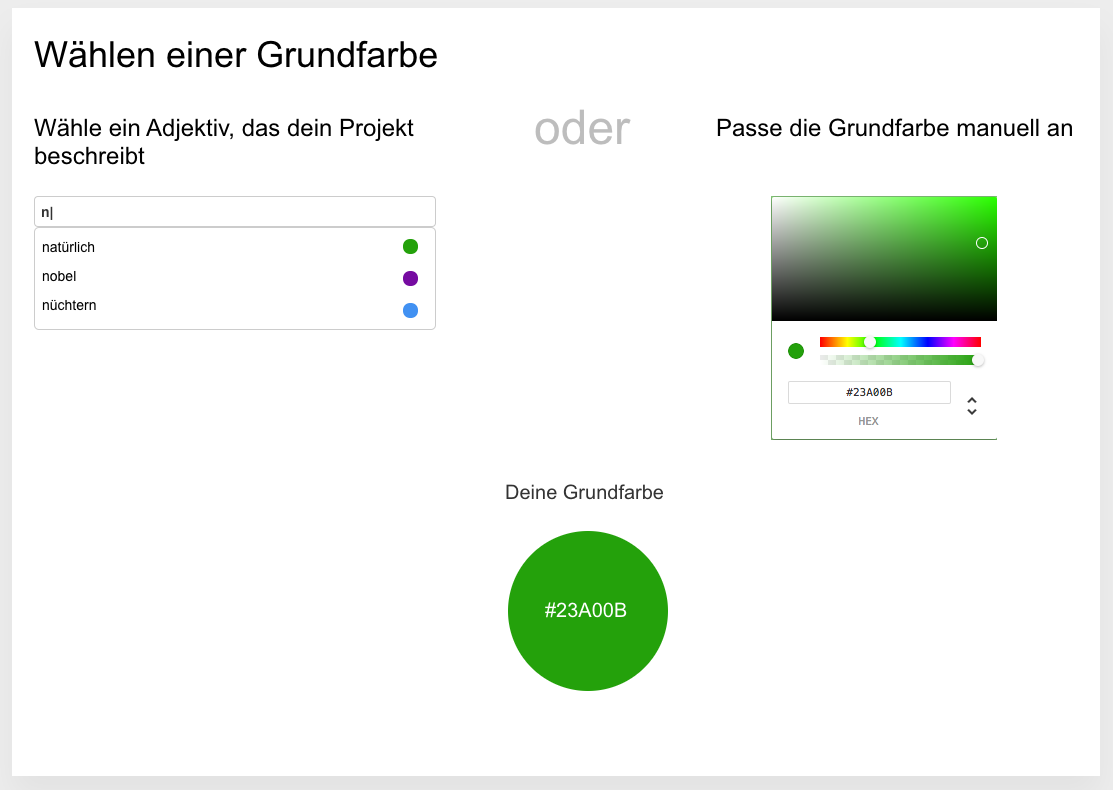
\includegraphics[width=1\textwidth]{images/wireframe-base-color.png}
    \caption{Mögliche Umsetzung der Wahl einer Grundfarbe}
    \label{fig:wire-base-color}
\end{figure}

\subsection{Finden einer Akzentfarbe}
Zum Finden einer Akzentfarbe müssen nun entweder Abstufungen der Grundfarbe, eine zur Grundfarbe komplementäre Farbe oder zwei zur Komplementärefarbe benachbarte Farbtöne gefunden werden

Für die tatsächliche Berechnung im Tool müssen die verwendeten Farben in den HSL-Farbraum (Hue, Saturation, Lightness) konvertiert werden. In diesem Farbraum werden Farbtöne radial auf einem Zylinder angeordnet \cite{joblove1978color}.
Um die Komplementärfarbe einer gegebenen Grundfarbe zu finden, muss also nur die auf dem Kreis gegenüberliegende Farbe gefunden, der Winkel also um 180 \degree vergrößert werden. 
Ist die Grundfarbe zum Beispiel ein Grün mit dem HEX-Wert \#23A00B würde dieses zunächst in den HSL-Farbraum konvertiert und die Werte H = 110\degree, S=87\% und L=43\% ergeben. \textit{Saturation} und \textit{Lightness} werden beibehalten, der \textit{Hue}-Wert wird um 180\degree erhöht. Die Komplementärfarbe hat also die Werte  H = 290\degree, S=87\% und L=43\% oder \#AD0ECD.

Soll ein triadisches Farbschema verwendet werden ist, das Vorgehen ähnlich. Hier muss jedoch von der errechenten Komplementärfarbe eine Abstufung im \textit{Hue}-Wert in beide Richtungen gefunden werden. Ein genauer Wert ist schwer zu bestimmen, jedoch liefert eine Abweichung von 30\% in beide Richtungen befreidigende Ergebnisse.\\
Die Komplementärfarbe mit den Werten  H = 290\degree, S=87\% und L=43\% würde also die zwei Abstufungen H = 260\degree, S=100\%, L=50\% und H = 320\degree, S=100\%, L=50\% bzw. \#4E0ECD und \#CD0E8D ergeben.

Um ein monochromatisches Farbschema zu erzeugen, können die \textit{Saturation}- und \textit{Lightness}-Werte verändert werden. Hier bieten sich viele Möglichkeiten, in diesem Beispiel wurden zum Erzeugen von drei Abstufungen zunächst die \textit{Saturation} um 40\% verringert, die \textit{Lightness} um 40\% erhöht und die \textit{Lightness} um 20\% verringert.\\
Die verschiedenen erstellten Farbschemata können Abb. \ref{fig:color-schemes} auf Seite \pageref{fig:color-schemes} entnommen werden. 

\begin{figure}[h]
    \centering
    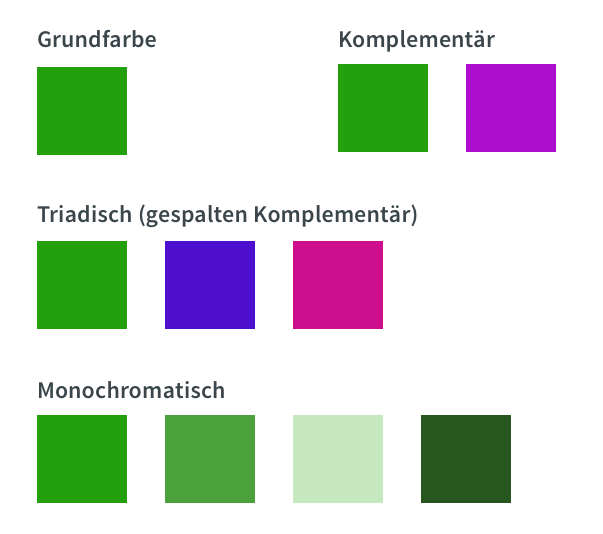
\includegraphics[width=1\textwidth]{images/color-schemes.png}
    \caption{Beispielhaft errechnete Farbpaletten}
    \label{fig:color-schemes}
\end{figure}

Da das Finden der Akzentfarbe ein recht geradliniger Prozess ist fällt es schwer, dem Nutzer hier über die Wahl des von ihm präferierten Farbschemas hinaus viel Interaktivität zu bieten.

\subsection{Komplettieren der Farbpalette}

Nachdem Grund- und Akzentfarbe gefunden sind, fehlen für eine nutzbare Farbpalette noch Grautöne.  Hier sollte darauf geachtet werden, nicht zu viele Grautöne zu verwenden, die sich nur marginal unterscheiden. In den meisten Fällen sollten 2-3 Grautöne in verschiedenen Abstufungen ausreichend sein.
Als einfachste Methode würde es sich anbieten, neutrale Grautöne ohne andere Farben zu wählen. Welche Grautöne genau genutzt werden muss dabei Subjektiv entschieden werden. Denkbar wären zum Beispiel \#eeeeee und \#666666.

\cite{elizabeth2016simple} erläutert eine andere Methode: Bei dieser Methode wird die Grundfarbe mit in die Grautöne eingearbeitet, was ein harmonischeres Bild erzeugt.  Für die Berechnung dieser Werte muss jedoch auf eine externe Bibliothek zurückgegriffen werden.

Hier sollte der Nutzer viele Freiheiten haben, das Tool sollte lediglich kontrollieren, ob die gewählten Grautöne innerhalb einiger Parameter liegen. So kann zum Beispiel über den \textit{Lightness}-Wert des HSL-Farbraumes überprüft werden, ob sich zwei Grautöne deutlich genug unterscheiden. Ebenso kann über den \textit{Saturation}-Wert sicher gestellt werden, dass die Grautöne nicht zu farbig sind.

%----------------------------------------------------------------------------------------

\section{Android \& iOS}\label{androidios}

Für beide Betriebssyteme liegen Guidelines bezüglich der visuellen Gestaltung, auch im Bezug auf Farben, vor. An diese soll sich auch das Tool halten. Das Tool soll hier aber nicht auf diese Guidelines verweisen oder sie wiederholen, sondern eine interaktive Möglichkeit bieten, auch für diese Plattformen eine Farbpalette zu erstellen.

Die Android Guidelines geben zwar keine zwingenden Farben vor, jedoch bieten sie eine große Vorauswahl an Farben, die verwendet werden können. Alle diese Farben sind mit einem Indikator für die Helligkeit versehen, die Guidelines Empfehlen die Farben mit der Helligkeit 500 als Grundfarbe zu benutzen. Hiervon bilden sich dann hellere und dunklere Varianten, die für andere Elemente verwendet werden.
Die Guidelines stellen außerdem eine Menge von Akzentfarben bereit, die frei mit einer der Grundfarben kombiniert werden können. Die Akzentfarbe sollte vor allem für interaktive Elemente verwendet werden.

Die Empfehlung der Farben, basierend auf Adjektiven, kann für Android-Porojekte weiterhin verwendet werden, jedoch mit einer limitierteren Farbauswahl. Akzentfarben müssen nicht mehr errechnet werden, hier kann dem Nutzer eine Auswahl der spezifizierten Akzentfarben gegeben werden, von der er eine auswählen kann.

Die iOS-Richtlinien sind deutlich weniger konkret. Unter iOS wird Farbe vor allem dafür genutzt, Interaktivität deutlich zu machen. Die guidelines schlagen hier 8 Farben vor, die auch dem Nutzer des Tools zur Auswahl gegeben werden sollten. Das Finden einer Akzentfarbe und von Grautönen entfällt dabei komplett. Das Vorschlagen der Farben auf Basis von Adjektiven wäre aber weiterhin, wenn auch recht limitiert, umsetzbar.



% Chapter 5

\chapter{Fazit} % Main chapter title

\label{Fazit} % For referencing the chapter elsewhere, use \ref{Aufgabenstellung} 

\lhead{\chaptername{} \thechapter{} - \emph{Fazit}} % This is for the header on each page - perhaps a shortened title

Abschließend lässt sich die Zielsetzung als erreicht ansehen. \\
Es wurden relevante Themengebiete für die Konzeption eines Tools definiert. In diesen Themengebieten wurden Regeln festgehalten, die auch für eine spätere programmatische Umsetzung verwendet werden können. In machen Gebieten, wie der Typographie oder den Farben, lassen diese Regeln mehr Spielraum für Interaktivität zu, in Anderen, wie beispielsweise den Interaktiven Elementen und Bildern, weniger. Lediglich im Bereich Whitespace konnten keinerlei Regeln definiert werden.

Mögliche Ideen für eine Umsetzung wurden in Form von Wireframes festgehalten und im Bereich der Typographie konnte mit Hilfe eines \textit{Proof of Concepts} gezeigt werden, dass auch eine tatsächliche technische Umsetzung mit moderatem Aufwand durchaus möglich ist.

Während des Projektes konnte aber auch festgestellt werden, dass das Übertragen von eher subjektiven Regeln für die Gestaltung von Artefakten in eine objektive, maschinenlesbare Form nicht einfach ist. Viele Entscheidungen, die Designer jeden Tag treffen, kann ein Computer nicht nachvollziehen. Auch können getroffene Entscheidungen nicht einfach als richtige oder falsche Referenzwerte übergeben werden, da deren Richtigkeit stark situationsabhängig ist. \\
Hier stellt sich die Frage, ob der Bereich \textit{Machine Learning} eine sinnvolle Ergänzung für das Projekt bieten könnte, also ob ein Computer, ähnlich wie ein Mensch, ein \textit{Gefühl} für eine gute oder schlechte Gestaltung entwickeln kann, wenn seine Datengrundlage groß genug ist.

Weiterhin ist auch die Frage nach dem tatsächlichen Nutzen den Tools noch ungeklärt. Zwar wird deutlich, das ein solches Tool eine gewisse Relevanz hat und auch umgesetzt werden kann, es kann jedoch nicht Festgestellt werden, ob das Tool dem Nutzer einen tatsächlichen Mehrwert liefern würde. Hierfür wären Nutzertests mit Prototypen nötig. 


\clearpage

%----------------------------------------------------------------------------------------
%	THESIS CONTENT - APPENDICES
%----------------------------------------------------------------------------------------

%----------------------------------------------------------------------------------------
%	THESIS CONTENT - APPENDICES
%----------------------------------------------------------------------------------------

\addtocontents{toc}{\vspace{2em}} % Add a gap in the Contents, for aesthetics

\appendix % Cue to tell LaTeX that the following 'chapters' are Appendices

% Include the appendices of the thesis as separate files from the Appendices folder
% Uncomment the lines as you write the Appendices

%% Appendix A

\chapter{Anforderungen} % Main appendix title

\label{anhangA} % For referencing this appendix elsewhere, use \ref{AppendixA}

\lhead{Anhang A. \emph{Anforderungen}} % This is for the header on each page - perhaps a shortened title

\section{Ursprüngliche Anforderungen}
\label{uanforderungen}

%\input{Appendices/AppendixB}
%\input{Appendices/AppendixC}

\addtocontents{toc}{\vspace{2em}} % Add a gap in the Contents, for aesthetics

\backmatter

\clearpage


%----------------------------------------------------------------------------------------
%	BIBLIOGRAPHY
%----------------------------------------------------------------------------------------

%----------------------------------------------------------------------------------------
%	BIBLIOGRAPHY
%----------------------------------------------------------------------------------------

\label{Literaturverzeichnis}

\bibliographystyle{plainnat} % Use the "unsrtnat" BibTeX style for formatting the Bibliography

\bibliography{Bibliography} % The references (bibliography) information are stored in the file named "Bibliography.bib"

\lhead{\emph{Literaturverzeichnis}} % Change the page header to say "Bibliography"

\clearpage

%----------------------------------------------------------------------------------------
%	DECLARATION PAGE
%	Your institution may give you a different text to place here
%----------------------------------------------------------------------------------------

%%----------------------------------------------------------------------------------------
%	DECLARATION PAGE
%	Your institution may give you a different text to place here
%----------------------------------------------------------------------------------------

\Declaration{

\addtocontents{toc}{\vspace{1em}} % Add a gap in the Contents, for aesthetics

\vspace*{2cm}

Ich versichere, die von mir vorgelegte Arbeit selbständig verfasst zu haben. Alle Stellen, die wörtlich oder sinngemäß aus veröffentlichten oder nicht veröffentlichten Arbeiten anderer entnommen sind, habe ich als entnommen kenntlich gemacht. Sämtliche Quellen und Hilfsmittel die ich für die Arbeit benutzt habe, sind angegeben. Die Arbeit hat mit gleichem Inhalt bzw. in wesentlichen Teilen noch keiner anderen Prüfungsbehörde vorgelegen.\\

\vspace*{2cm}
 
\rule[1em]{25em}{0.5pt}\\ % This prints a line for the signature

\vspace*{-1.2cm}

Datum, Ort\\

\vspace*{1.5cm}

\rule[1em]{25em}{0.5pt}\\ % This prints a line to write the date

\vspace*{-1.2cm}

Unterschrift\\
}

\clearpage % Start a new page

\end{document}
